\subsection{Mixed Integer Non Linear Programming Formulations}\label{Form}
% \JP{In this section we present a MINLP formulation for the (\AMD). Let us denote by $\mathcal T$ the set of stages/tasks that the mothership and the fleet of drones have to carry out. These stages are visits to the different graphs in $\mathcal G$ with the required constraints. A stage $t\in\mathcal O$ is referred to as the operation in which the mothership launches some drones from a taking-off location, denoted by $x_L^o$ and later it takes them back on a rendezvous location $x_R^o$. Here, it is important to realize that both locations $x^L_t$ and $x^R_t$ must be determined in the continuous space where the mothership is assumed to move. Note that $|\mathcal T|\leq|\mathcal G|$, since it is assumed that, for each stage, at least one drone must be launched. Clearly, the distance $d_{LR}^o$ traveled by the base vehicle for the stage $t$, i.e., to go from $x_L^o$ to $x_R^o$ is
% $$d_{LR}^o=\|x_L^o - x_R^o\|,$$
% where $\|\cdot\|_2$ denoted the Euclidean distance,  although this assumption can be extended to any $l_p$ norm, $1\leq p\leq \infty$.} 
The purpose of this section is to present a Mixed Integer Non-Linear Programming formulation for the \AMD \ that can be applied to solve instances of this problem.

In Subsection \ref{subsection:desc}, we mention that the mothership can move without any restriction in a continuous space that for simplicity is supposed to be $\mathbb R^2$. Although it is possible to measure distances with any $l_p$-norm, $1\leq p\leq \infty$ (see \cite{Blanco2017}), for the sake of presentation, in this work the distances are measured by the Euclidean norm ($p= 2$).

First of all, we introduce the parameters or initial data that formally describe the problem and that are summarized in Table \ref{table:t1}.

%  \begin{table}[!h]
% \scriptsize
% \centering
% \begin{tabular}{ | l | }
% \hline
% \textbf{Problem Parameters}\\
% \hline
% $orig$: coordinates of the point defining the origin of the mothership path (or tour).\\
% $dest$: coordinates of the point defining the destination of the mothership path (or tour).\\
% $\mathcal{T}=\mathcal{U}\cup\mathcal{P}$: set of targets.
% $\mathcal{U}$: set of points.
% $\mathcal{P}$: set of polygonal chains.\\
% $q = (q(x_1), q(x_2))\in \mathbb R^2$: coordinates of the point $q\in\mathcal U$.\\
% $p = (V_p, S_p)$: set of endpoints and segments of each polygonal chain $p \in \mathcal{P}$.\\
% $\mathcal L (p)$: total length of the polygonal chain $p \in \mathcal{P}$.\\
% $\mathcal{L}(s_p)$: length of segment $s_p$ of the polygonal $p \in \mathcal{P}$.\\
% $A^{v_p}$: coordinates of the point $v_p$ of the polygonal $p \in \mathcal{P}$.\\
% $\alpha^{p}$: percentage of the polygonal $p \in \mathcal{P}$ that must be visited.\\
% $v_D$: drone speed.\\
% $v_M$: mothership speed.\\
% $N$: drone endurance. \\
% $M$: big-M constant.\\
% \hline
% \end{tabular}
% \caption{Nomenclature for AMMDRPG}
% \label{table:t1}
% \end{table}

% Please add the following required packages to your document preamble:
% \usepackage{graphicx}
\begin{table}[]
\centering
\resizebox{\textwidth}{!}{%
\begin{tabular}{|c|c|l|}
\hline
\multicolumn{3}{|l|}{\textbf{Problem Parameters}} \\ \hline
\textbf{P. Name} & \textbf{Range} & \textbf{Description} \\ \hline
$orig$ & $\mathbb R^2$ & Coordinates of the point defining the origin of the mothership path (or tour). \\ \hline
$dest$ & $\mathbb R^2$ & Coordinates of the point defining the destination of the mothership path (or tour). \\ \hline
$\mathcal{A}$ & $\{1,\ldots,|\mathcal A|\}$ & Set of points. \\ \hline
$\mathcal{P}$ & $\{1, \ldots,|\mathcal P|\}$ & Set of polygonal chains. \\ \hline
$\mathcal{T}=\mathcal{A}\cup\mathcal{P}$ & $\{1, \ldots, |\mathcal T|\}$ & Set of targets. \\ \hline
$a=(a(x_1), a(x_2))$ & $\mathbb R^2$ & Coordinates of the point $a\in\mathcal A$. \\ \hline
$p = (V_p, S_p)$ & $\mathbb R^2$ & Set of breakpoints and segments of each polygonal chain $p\in\mathcal P$. \\ \hline
$V = \mathcal A \cup \left(\bigcup_{p\in\mathcal P} V_p\right)$ & $\mathbb R^2$ & Set of target points and set of breakpoints of polygonal targets. \\ \hline
$\mathcal L (p)$ & $\mathbb R_+$ & Total length of the polygonal chain $p \in \mathcal{P}$. \\ \hline
$\mathcal L(s_p)$ & $\mathbb{R}_+$ & Length of the segment $s_p$ of the polygonal chain $p\in\mathcal P$. \\ \hline
$A^{v_p}$ & $\mathbb R^2$ & Coordinates of the point $v_p$ of the polygonal $p\in\mathcal P$. \\ \hline
$\alpha^p$ & $[0, 1]$ & Percentage of the polygonal $p\in\mathcal P$ that must be visited. \\ \hline
$v_D$ & $\mathbb R_+$ & Drone speed. \\ \hline
$v_M$ & $\mathbb R_+$ & Mothership speed. \\ \hline
$N$ & $\mathbb R_+$ & Drone endurance. \\ \hline
$M$ & $\mathbb R_+$ & Big-M constant. \\ \hline
$m$ & $\mathbb R_+$ & Small-M constant. \\ \hline
\end{tabular}%
}
\caption{Nomenclature for the Multitarget-MDRP}
\label{table:t1}
\end{table}

\begin{table}[]
\scriptsize
\caption{Summary of binary variables used in the mathematical programming model\label{table:t2}}
\begin{tabular}{|c|c|c|l|}
\hline
\multicolumn{4}{|l|}{\textbf{Binary Decision Variables}} \\ \hline
\textbf{Name} & \textbf{Set} & \textbf{Domain} & \multicolumn{1}{c|}{\textbf{Description}} \\ \hline
$\mu_R^{s_p}$ & $s_p\in S_p:p\in\mathcal P$ & Binary & \begin{tabular}[c]{@{}l@{}}1, if the entry point on the polygonal chain is located in the line segment $s_p$,\\ 0, otherwise.\end{tabular} \\ \hline
$\mu_L^{s_p}$ & $s_p\in S_p:p\in\mathcal P$ & Binary & \begin{tabular}[c]{@{}l@{}}1, if the exit point on the polygonal chain is located in the line segment $s_p$,\\ 0, otherwise.\end{tabular} \\ \hline
$z_{\mathcal P}^{s_ps'_p}$ & $s_p, s'_p\in S_p:p\in\mathcal P$ & Binary & \begin{tabular}[c]{@{}l@{}}1, if the entry and  exit points are located in the line segments $s_p$ and $s'_p$, respectively,\\ 0, otherwise.\end{tabular} \\ \hline
$u^{to}$ & $t\in \mathcal T, o\in\mathcal O$ & Binary & \begin{tabular}[c]{@{}l@{}}1, if the drone starts the operation $o$ in the target $t$,\\ 0, otherwise.\end{tabular} \\ \hline
$v^{to}$ & $t\in\mathcal T,o\in\mathcal O$ & Binary & \begin{tabular}[c]{@{}l@{}}1, if the drone finishes the operation $o$ in the target $t$,\\ 0, otherwise.\end{tabular} \\ \hline
$\delta^{to}$ & $t\in\mathcal T,o\in\mathcal O$ & Binary & \begin{tabular}[c]{@{}l@{}}1, if the drone visits the target $t$ in the operation $o$,\\ 0, otherwise.\end{tabular} \\ \hline
$y^{tt'o}$ & $t,t'\in\mathcal T,o\in\mathcal O$ & Binary & \begin{tabular}[c]{@{}l@{}}1, if the drone goes from the target $t$ to the target $t'$ in the operation $o$,\\ 0, otherwise.\end{tabular} \\ \hline
\end{tabular}
\end{table}


\begin{table}[]
\scriptsize
\caption{Summary of continuous variables used in the mathematical programming model\label{table:t3}}
\begin{tabular}{|c|c|c|l|}
\hline
\multicolumn{4}{|l|}{\textbf{Continuous Decision Variables}} \\ \hline
\textbf{Name} & \textbf{Set} & \textbf{Domain} & \multicolumn{1}{c|}{\textbf{Description}} \\ \hline
$R^t$ & $t\in\mathcal T$ & $\mathbb R^2$ & \begin{tabular}[c]{@{}l@{}}Coordinates representing the entry point on the target $t$. \\ If the target is a point, it coincides with $L^t$.\end{tabular} \\ \hline
% $\rho$ & $\mathcal P$ & $[0, |S_p|]$ & Parameterization of the entry point $R$ on the polygonal chain. \\ \hline
$\gamma_R^{v_p}$ & $v_p\in V_p:p\in\mathcal P$ & $[0, 1]$ & Parameterization of the entry point $R^p$ on the segment $s_p=\overline{v_p(v+1)_{p}}$ of the polygonal chain. \\ \hline
$L^t$ & $t\in\mathcal T$ & $\mathbb R^2$ & \begin{tabular}[c]{@{}l@{}}Coordinates representing the exit point on each target. \\ If the target is a point, it coincides with $R^t$.\end{tabular} \\ \hline
% $\lambda$ & $\mathcal P$ & $[0, |S_p|]$ & Parameterization of the exit point $L$ on the polygonal chain. \\ \hline
$\gamma_L^{v_p}$ & $v_p\in V_p:p\in\mathcal P$ & $[0, 1]$ & Parameterization of the exit point $L^p$ on the segment $s_p=\overline{v_p(v+1)_{p}}$ of the polygonal chain. \\ \hline
% $\nu_\text{min}$ & $\mathcal P$ & $[0, |S_p|]$ & Auxiliary variable used for linearizing the absolute value. \\ \hline
% $\nu_\text{max}$ & $\mathcal P$ & $[0, |S_p|]$ & Auxiliary variable used for linearizing the absolute value. \\ \hline
$x_L^o$ & $o\in\mathcal O$ & $\mathbb R^2$ & Coordinates representing the point where the mothership launches the drone at operation $o$. \\ \hline
$x_R^o$ & $o\in\mathcal O$ & $\mathbb R^2$ & Coordinates representing the point where the mothership retrieves the drone at operation $o$. \\ \hline
$d_L^{to}$ & $t\in\mathcal T, o\in\mathcal O$ & $\mathbb R_+$ & \begin{tabular}[c]{@{}l@{}}Distance travelled by the drone from the launching point $x_L^o$ on the mothership \\ to the first target point $R^t$ associated to the operation $o$.\end{tabular} \\ \hline
$d_\text{out}^{tt'}$ & $t,t'\in\mathcal T$ & $\mathbb R_+$ & \begin{tabular}[c]{@{}l@{}}Distance travelled by the drone from the launching point $L^t$ on one target \\ to the rendezvous point $R^{t'}$ on another one.\end{tabular} \\ \hline
$d_R^{to}$ & $t\in\mathcal T,o\in\mathcal O$ & $\mathbb R_+$ & \begin{tabular}[c]{@{}l@{}}Distance travelled by the drone from the launching point of the last visited target $L^t$ \\ to the rendezvous point $x_R^o$ associated to the operation $o$.\end{tabular} \\ \hline
$d_{LR}^o$ & $o\in\mathcal O$ & $\mathbb R_+$ & \begin{tabular}[c]{@{}l@{}}Distance travelled by the drone from the launching point $x_L^o$ \\ to the rendezvous point $x_R^o$ at operation $o$.\end{tabular} \\ \hline
$d_{RL}^o$ & $o\in\mathcal O\CV{\setminus \{|\mathcal O|\}}$ & $\mathbb R_+$ & \begin{tabular}[c]{@{}l@{}}Distance travelled by the mothership and the drone from the rendezvous point $x_R^o$ \\ at operation $o$ to the launching point $x_L^{o+1}$ at the operation $o+1$.\end{tabular} \\ \hline
$d_\mathcal{P}^{s_ps_p'}$ & $s_p,s_p'\in S_p:p\in\mathcal P$ & $\mathbb R_+$ & \begin{tabular}[c]{@{}l@{}}Distance travelled by the drone from the exit point on the segment $s_p$ on one polygonal \\ to the entry point on the segment $s_p'$ of the same polygonal.\end{tabular} \\ \hline
$d_\text{in}^t$ & $t\in\mathcal T$ & $\mathbb R_+$ & \begin{tabular}[c]{@{}l@{}}Distance travelled by the drone from the rendezvous point $R^t$ \\ to the launching point $L^t$ on the same target.\\ If the target is a point, this distance is 0.\end{tabular} \\ \hline
\end{tabular}
\end{table}

% \begin{table}[h!]
% %\tiny
% \scriptsize
% \centering
% \begin{tabular}{|l|}
% \hline 
% \textbf{Binary and Integer Decision Variables}\\
% \hline
% $\text{entry}^p \in \{0,1\},$  $\forall p \in \mathcal P$ : auxiliary binary variable used for linearizing the absolute value in the constraints.\\
% $\mu_R^{s_p}, \mu_L^{s_p} \in \{0, 1\},$ $\forall s_p \in \mathcal S_p$ ($p\in\mathcal P$): equal to 1 when $R^p$ (resp. $L^p$) is located in the line segment $s_p$ of the polygonal chain $p$
% $\mu_R^{s_p}, \mu_L^{s_p} \in \{0, 1\}, \:\: \forall s_p \in \mathcal S_p$ ($p\in\mathcal P$): equal to 1 when $R^p$ (resp. $L^p$) is located in the line segment $s_p$ of the polygonal chain $p$, \\\hspace*{1cm} 0 otherwise.\\
% $u^{to} \in \{0,1\}, \:\: \forall t \in \mathcal{T},\:\: \forall o \in \mathcal O$: equal to 1 if the drone enters in the target $t$ in the operation $o$, 0 otherwise.\\
% $v^{to} \in \{0,1\}, \:\: \forall t \in \mathcal T,\:\: \forall o \in\mathcal O$: equal to 1 if the drone exits from the target $t$ in the operation $o$, 0 otherwise.\\
% $\delta^{to} \in \{0, 1\}, \:\: \forall t\in\mathcal T,\:\: \forall o\in\mathcal O$: equal to 1 if the target $t$ is included in the operation $o$.\\
% $y^{tt'o} \in \{0, 1\},  \:\: \forall t, t' \in \mathcal T,\:\: \forall o\in\mathcal O$: equal to 1 if the drone goes from the target $t$ to the target $t'$ in the operation $o$.\\
% \hline
% \textbf{Continuous Decision Variables}\\
% \hline
% $R^{t}, \:\: \forall t \in \mathcal T$: coordinates representing the entry point on the target $t$. If the target is a point, it coincides with $L^t$. \\
% $L^{t}, \:\: \forall t \in \mathcal T$: coordinates representing the exit point on the target $t$. If the target is a point, it coincides with $R^t$.\\
% $\rho^{p} \in [0,|S_p|]$ and $\lambda^{p} \in [0,n_{|S_p|}], \:\: \forall p \in \mathcal P$: that models the parameterization of the entry (resp. exit) point on the polygonal chain $p$.\\
% $\gamma_R^{s_p}, \gamma_L^{s_p}, \:\: \forall s_p\in\mathcal S_p$ ($p \in \mathcal P$): continuous variable in $[0,1]$ that represents the parameter value of the $R^p$ (resp. $L^p$) \\
% \hspace*{1cm} variable in the line segment $s_p$ of the polygonal chain $p$.\\
% $\nu_\text{min}^{p}$ and $\nu_\text{max}^{p} \in [0,1], \forall p \in $ ($g \in \mathcal{G}$): auxiliary variables used for linearizing expressions.\\
% $x_L^o, \:\: \forall o \in\mathcal O$: coordinates representing the point where the mothership launches the drone at operation $o$.\\
% $x_R^o, \:\: \forall o \in\mathcal O$: coordinates representing the point where the mothership retrieves the drone at operation $o$.\\
% $d_L^{to} \geq 0, \:\: \forall t \in\mathcal T, \:\:\forall o\in\mathcal O$: representing the distance travelled by the drone from the launching\\
% \hspace*{1cm} point $x_L^o$ on the mothership to the first target point $R^t$ associated to the operation $o$.\\
% $d^{tt'} \geq 0, \:\: \forall t, t' \in \mathcal T $: representing the distance travelled by the drone from the launching\\
% \hspace*{1cm} point $L^t$ on $t$ to the rendezvous point $R^{t'}$ on $t'$.\\
% $d^{t} \geq 0, \:\: \forall t \in \mathcal T$: representing the distance travelled by the drone from the rendezvous\\
% \hspace*{1cm} point $R^{t}$ to the launching point $L^{t}$ on $t$.\\
% $d_R^{to} \geq 0, \:\: \forall t \in\mathcal T, \:\:\forall o\in\mathcal O$: representing the distance travelled by the drone from the last visited point $L^t$\\
% \hspace*{1cm} to the rendezvous point $x_R^o$ associated to the operation $o$.\\
% $d_{LR}^o \geq 0, \:\: \forall o \in\mathcal O$: representing the distance travelled by the mothership from the \\
% \hspace*{1cm} launching point $x_L^o$ to the rendezvous point $x_R^o$ at stage $t$.\\
% $d_{RL}^o \geq 0, \:\: \forall o \in\mathcal O$: representing the distance travelled by the mothership from the \\ 
% \hspace*{1cm} rendezvous point $x_R^o$ at operation $o$ to the launching point $x_L^{(o+1)}$ at the operation $o+1$.\\
% \hline
% \end{tabular}
% \caption{Decision Variables for AMMDRPG}
% \label{table:t2}
% \end{table}


To represent the movement of the drone within a polygonal $p\in\mathcal P$, we proceed to introduce some notation related to $p$.
Let $p = (V_p, S_p)$ be a polygonal chain in $\mathcal P$ whose total length is denoted by $\mathcal L(p)$. Here, $V_p$ denotes the set of vertices and $S_p$ denotes the set of segments connecting pairs of consecutive vertices whose cardinality is $|S_p|$. Let $s_p=\overline{v_p(v+1)_p}$ be the segment $s$ of the polygonal $p \in \mathcal P$ and let $\mathcal  L(s_p)$ be its length. Since we need to refer to interior points of the segment $s_p$, these continuum of points is parameterized by the two endpoints $A^{v_p}= (A^{v_p}(x_1), A^{v_p}(x_2))$ and $A^{(v+1)_p}= (A^{(v+1)_p}(x_1), A^{(v+1)_p}(x_2))$ of the segment: $x\in[A^{v_p}, A^{(v+1)_p}]$ if and only if $\exists \:\: \gamma\in[0, 1]$ such that $x=\gamma A^{v_p} + (1-\gamma)A^{(v+1)_p}$. Hence, the length of the segment $s_p$ is $\mathcal L(s_p) =\|A^{v_p} -  A^{(v+1)_p}\|$.

Next, we need to determine the placement of the entry point, $R^p$, on the polygonal chain $p$ introducing the following inequalities for each $p\in\mathcal P$:

\begin{equation}\label{P-C}\tag{$\mathcal P$-C}
\small
 R^p\in p \Longleftrightarrow
 \left\{
 \begin{array}{cclr}
 \gamma_R^{1_p}                     & \leq & \mu_R^{1_p},                                  & \\
 \gamma_R^{s_p}                     & \leq & \mu_R^{s_p-1} + \mu_R^{s_p}, & s_p\in S_p \setminus\{1\},\\
 \gamma_R^{|V_p|_p}             & \leq & \mu_R^{|S_p|_p}, \\
 \displaystyle\sum_{s_p\in S_p} \mu_R^{s_p}      &   =  & 1, & \\
 \displaystyle\sum_{v_p\in V_p} \gamma_R^{v_p}   &   =  & 1, & \\
  R^p                               & = & \displaystyle\sum_{v_p\in V_p}\gamma_R^{v_p}A^{v_p}. & \\
 \end{array}
 \right.
\end{equation}

The first, second and third inequalities link $\mu_R^{s_p}$ and $\gamma_R^{s_p}$ variables: they state that the variable $\gamma_R^{s_p}$ that gives the representation of a point $R^p$ on the line segment $s_p$ is active (non-null) only if this line segment is chosen to enter in polygonal $p$, i.e., $\mu_R^{s_p}=1$. The fourth equation sets that only one line segment is chosen for entering each polygonal chain. Finally, the fifth and sixth equations set the representation of $R^p$ as a convex combination of the extreme points of the selected line segment.
In the same way, we can model the location of the exit point, $L^p$, by using the variables $L^p$, $\mu_L^{s_p}$ and $\gamma_L^{s_p}$ explained in Table \ref{table:t2} and Table \ref{table:t3}, respectively.

% We shall refer to $e_g$  as a generic edge $e$ of this graph $g$. The  edge $e_g$ is determined by its endpoints $B^{e_g}, C^{e_g}$ and its length $\|\overline{B^{e_g}C^{e_g}}\|$ is denoted by $\mathcal L(e_g)$. For each edge $e_g$, we assign a binary variable $\mu^{e_g}$ that indicates whether or not the drone visits $e_g$. In addition, for each edge $e_g$ we define an entry $(R^{e_g}, \rho^{e_g})$ and an exit point $(L^{e_g}, \lambda^{e_g})$, being $\rho^{e_g}$ and $\lambda^{e_g}$ the values in the parametrization of the edge $e_g$ where the drone enters and leaves the edge. \\



\bigskip

% \bigskip
% \noindent
% \CV{In both cases the corresponding constraints are nonlinear. In order to linearize them, we need to introduce a binary variable} $\text{entry}^{e_g}$ that determines the traveling direction on the edge $e_g$ as well as the definition of the parameter values $\nu_\text{min}^{e_g}$ and $\nu_\text{max}^{e_g}$ of the access and exit points to that segment. Then, for each edge $e_g$, the absolute value constraint \eqref{eq:alphaE} can be represented by:

% \begin{equation}\label{eq:alpha-E}\tag{$\alpha$-E}
%  \mu^{e_g}|\rho^{e_g}-\lambda^{e_g}|\geq \alpha^{e_g} \Longleftrightarrow
%  \left\{
%  \begin{array}{ccl}
%   \rho^{e_g} - \lambda^{e_g}                       & =    & \nu_\text{max}^{e_g} - \nu_\text{min}^{e_g}                                     \\
%   \nu_\text{max}^{e_g}                         & \leq & 1-{\text{entry}^{e_g}}                                    \\
%   \nu_\text{min}^{e_g}                      & \leq & {  \text{entry}^{e_g}},                                        \\
%   \mu^{e_g}(\nu_\text{max}^{e_g} + \nu_\text{min}^{e_g} ) & \geq & \alpha^{e_g}
%   \\
%  \end{array}
%  \right.
% \end{equation}

% \noindent
% The linearization of \eqref{eq:alphaG} is similar to \eqref{eq:alphaE} by changing the last inequality in \eqref{eq:alpha-E} for

% \begin{equation}\label{eq:alpha-G}\tag{$\alpha$-G}
% \sum_{e_g\in E_g} \mu^{e_g}(\nu_\text{max}^{e_g} + \nu_\text{min}^{e_g})\mathcal L(e_g)\geq \alpha_g\mathcal L(g).
% \end{equation}

In our approach to model the \AMD \ we use operations identified with the order in which the different elements in the problem are visited. Let us denote by $\mathcal O$ the set of operations that the mothership and the drone have to carry out. An operation $o\in\mathcal O$ is referred to as the one in which the mothership launches a drone from a taking-off location, denoted by $x_L^o$ and later it takes it back on a rendezvous location $x_R^o$. Each operation consists on the drone visit to one or more targets in $\mathcal T$ with the required constraints. At this point, it is relevant to note that the pair of locations $x_L^o$ and $x_R^o$ must be selected in the plane where the mothership is presumed to move. Observe that $|\mathcal O|\leq|\mathcal T|$ because of the assumption that at least one target is visited for each operation.

% According to the notation introduced above, we write this generic path in the following form:

% $$
% x_L^o\rightarrow R^{p}\rightarrow L^{e_g}\rightarrow\ldots\rightarrow R^{e^\prime_g}\rightarrow L^{e^\prime_g}\rightarrow \ldots \rightarrow R^{e''_g} \rightarrow x_R^o\rightarrow x_L^{t+1}.
% $$

%{\bf \color{atomictangerine} ************************ 

%TO BE INSERTED: An example showing the notation with a figure...

%     ************************}
     
Figure \ref{fig:Fig1} shows an example of problem instance with 4 polygonal targets. The point $orig$ from where the mothership together with the drone must start their tour, is located in the origin, while the destination point $dest$ is the point (100,100).
    
     
\pgfplotsset{compat=1.15}

\begin{figure}
\centering
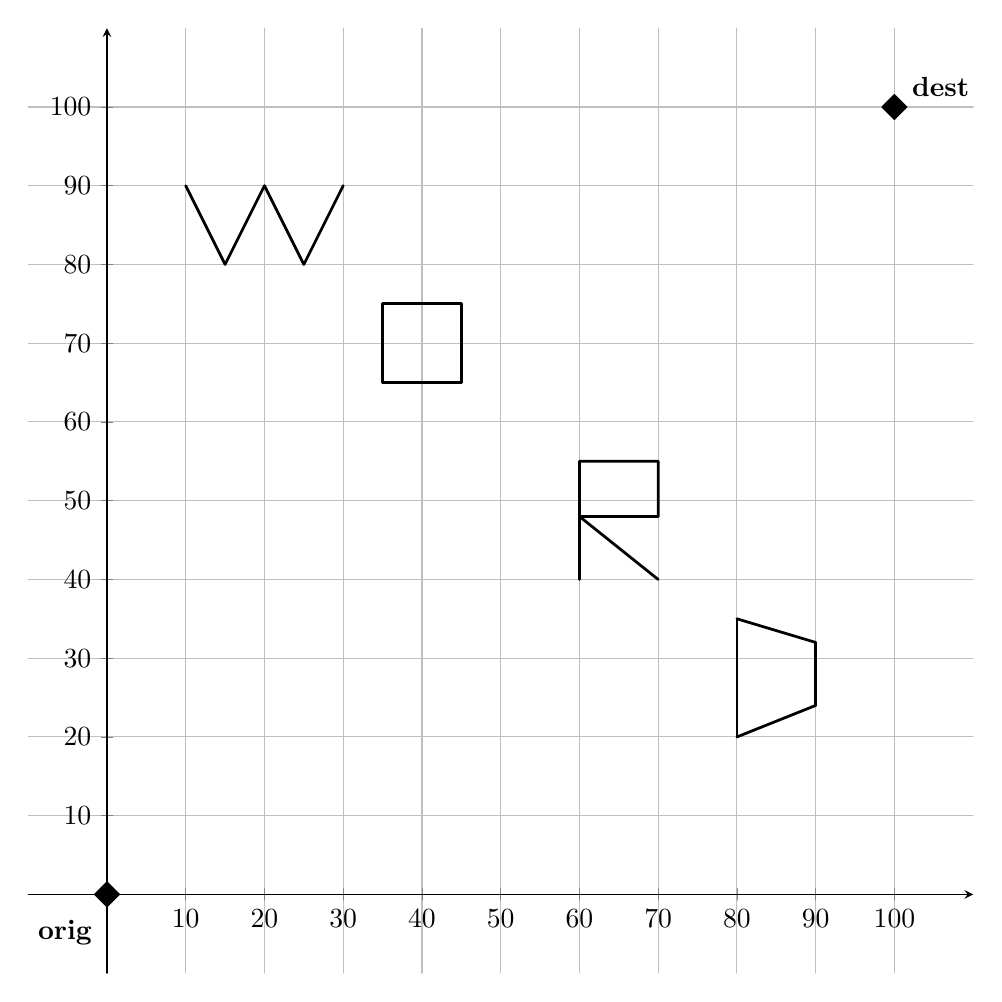
\begin{tikzpicture}[line cap=round,line join=round,>=triangle 45,x=1cm,y=1cm]
\begin{axis}[
x=0.1cm,y=0.1cm,
axis lines=middle,
ymajorgrids=true,
xmajorgrids=true,
xmin=-10,
xmax=110,
ymin=-10,
ymax=110,
xtick={0,10,...,100},
ytick={0,10,...,100},]
%\clip(-86.54891610135228,-35.76340486396641) rectangle (196.61700168770358,127.62998372971737);
%\fill[line width=2pt] (0,100) -- (0,0) -- (100,0) -- (100,100) -- cycle;
%\fill[line width=2pt] (35,75) -- (35,65) -- (45,65) -- (45,75) -- cycle;
%\fill[line width=2pt] (80,35) -- (80,20) -- (90,24) -- (90,32) -- cycle;
\draw [line width=1pt] (10,90)-- (15,80)-- (20,90)-- (25,80)-- (30,90);
\draw [line width=1pt] (35,75)-- (35,65);
\draw [line width=1pt] (35,65)-- (45,65);
\draw [line width=1pt] (45,65)-- (45,75);
\draw [line width=1pt] (45,75)-- (35,75);
\draw [line width=1pt] (60,40)-- (60,55)-- (70,55)-- (70,48)-- (60,48)-- (70,40);
\draw [line width=1pt] (80,35)-- (80,20);
\draw [line width=1pt] (80,20)-- (90,24);
\draw [line width=1pt] (90,24)-- (90,32);
\draw [line width=1pt] (90,32)-- (80,35);
\draw (-10,-2) node[anchor=north west] {$\mathbf{orig}$};
\draw (101,105) node[anchor=north west] {$\mathbf{dest}$};
\begin{scriptsize}
\draw [fill=black] (0,0) ++(-4.5pt,0 pt) -- ++(4.5pt,4.5pt)--++(4.5pt,-4.5pt)--++(-4.5pt,-4.5pt)--++(-4.5pt,4.5pt);
\draw [fill=black] (100,100) ++(-4.5pt,0 pt) -- ++(4.5pt,4.5pt)--++(4.5pt,-4.5pt)--++(-4.5pt,-4.5pt)--++(-4.5pt,4.5pt);
\end{scriptsize}
\end{axis}
\end{tikzpicture}
\caption{Example of problem instance with polygonal targets.}
\label{fig:Fig1}
\end{figure}
% \label{fig:Fig1}

To include the definition of the paths followed by the drone in our mathematical programming formulation we need to make decisions to choose:
\begin{itemize}
    \item The optimal assignment of the targets to each operation $o$.
    \item The optimal order to visit the targets for its corresponding operation $o$.
\end{itemize}

% Binary variables
% Thus, to this end one can define the following binary variables:

We can model the route followed by the drone using the binary variables $u^{to}$, $y^{tt'o}$, $\delta^{to}$ and $v^{to}$ defined in Table \ref{table:t2}.


% \begin{itemize}
%   \item $u^{{e_g}td} = 1$ if the visit of graph $g$ is done at stage $t$ by the drone $d$ and it starts from edge $e_g$.
%   \item $v^{{e_g}td}= 1$ if the visit of graph $g$ that is done by drone $d$ at stage $t$ finishes in the edge $e_g$.
%   \item $z^{e_ge'_g}= 1$ if the drone moves from edge $e_g$ to $e'_g$ while visiting the graph $g$.
% \end{itemize}

% By using these binary variables, we can model the route that follows the drone:
\begin{align}
    \sum_{t\in \mathcal T} u^{to} & \leq 1, &\forall o\in \mathcal O, \label{st:DEnt}\\%\tag{DEn}\\
    \sum_{t\in \mathcal T} v^{to} & \leq 1, &\forall o\in \mathcal O, \label{st:DExt}\\%\tag{DEx}\\
    \sum_{o\in \mathcal O} \delta^{to} & = 1, &\forall t\in \mathcal T, \label{st:DIn} \\
    \delta^{to} - u^{to} & = \sum_{t'\neq t} y^{t'to}, &\forall t\in \mathcal T,\:\forall o\in \mathcal O, \label{st:Dinu}\\
    \delta^{to} - v^{to} & = \sum_{t'\neq t} y^{tt'o}, &\forall t\in \mathcal T,\:\forall o\in \mathcal O, \label{st:Dinv}\\
    \sum_{t, t'\in S}y^{tt'o} & \leq |S|-1, &\forall S\subsetneq\mathcal T,\:\forall o\in\mathcal O.
    \label{st:SEC}
    % \sum_{e_g\in E_g} \sum_{t\in \mathcal T} \sum_{d\in\mathcal D} u^{to} & = 1, &\forall g\in\mathcal G \label{st:DEng}\\%\tag{D
    % \sum_{e_g\in E_g} \sum_{t\in \mathcal T} \sum_{d\in\mathcal D} v^{to} & = 1, &\forall g\in\mathcal G \label{st:DExg}\\%\tag{D
    % \sum_{e_g\in E_g} u^{to} & = \sum_{e_g\in E_g} v^{to}, &\forall g\in\mathcal G, \forall o\in \mathcal T, \forall d\in\mathcal D \label{st:Duv}\\%\tag{D
    % \sum_{e^\prime_g\in E_g} z_g^{e^\prime_ge_g} + \sum_{t\in \mathcal T} \sum_{d \in \mathcal D} u^{to} & = \mu^{e_g}, &\forall e_g\in E_g:g\in\mathcal G, \forall d\in\mathcal D \label{st:DInu}\\
    % \sum_{e^\prime_g\in E_g} z_g^{e_ge^\prime_g} + \sum_{t\in \mathcal T} \sum_{d \in \mathcal D} v^{to} & = \mu^{e_g}, &\forall e_g\in E_g:g\in\mathcal G \label{st:DInv}
\end{align}

Constraints \eqref{st:DEnt} and \eqref{st:DExt} state that for each operation the drone only can enter and exit, respectively, by one target.  Constraints \eqref{st:DIn} ensure that every target will be visited in some operation. Constraints \eqref{st:Dinu} assure that if target $t$ is visited by the drone for the operation $o$, one of two alternative conditions must take place: either $t$ is the first target for the operation $o$ or target $t$ is visited by the drone after visiting another target $t'$ for the operation $o$. Similarly, constraints \eqref{st:Dinv} state that if the target $t$ for the operation $o$ is visited by the drone, either $t$ is the last target of the operation, or the drone must move to another target $t'$ of the operation $o$ after visiting target $t$. Finally, inequalities \eqref{st:SEC} are the subtour elimination constraints applied to each operation. Note that, the complete family of SEC constraints can not be included to the model when we implement this formulation, because there is a exponential number of them and it can induce a memory problem on-the-shelf solvers. This problem can be solved by performing a row generation procedure that includes the constraints whenever they are needed by a separation oracle. To detect these SEC inequalities, as usual, we look for disconnected components in the current solution. Among them, we choose the shortest subtour found in the solution to be added as a lazy constraint to the model.\\

% Constraints \eqref{st:DInu} (resp. \eqref{st:DInv}) state that if the edge $e_g$ is visited, $\mu^{e_g}=1$, then either the drone enters coming from (leaves to) the mothership, $\sum_{t\in \mathcal T} \sum_{d \in \mathcal D} u^{to}=1$ ($\sum_{t\in \mathcal T} \sum_{d \in \mathcal D} v^{to}=1$), or it enters from (leaves to) another edge $e^\prime_g$, $\sum_{e^\prime_g\in E_g} z_g^{e^\prime_ge_g}=1$ ($\sum_{e^\prime_g\in E_g} z_g^{e_ge^\prime_g} =1$).

% A first attempt to model this problem uses stages identified with the order in which the different elements in the problem are visited. We identify each visit to one of the target graphs with a stage of the process. Then, by using the notation below, we define the stages set associated to graphs $T:=\{1,\ldots,|\mathcal G|\}$ and those associated to the launching and rendezvous points including $orig$ and $dest$ $T'=\{0,\ldots,|\mathcal G|+1\}$. For each stage $t\in T$, the drone follows the following path starting from the mothership, visiting the required edges of $g$ and returning to the mothership:

% $$
% x_L^o\rightarrow R^{e_g}\rightarrow L^{e_g}\rightarrow\ldots\rightarrow R^{e^\prime_g}\rightarrow L^{e^\prime_g}\rightarrow \ldots \rightarrow R^{e''_g} \rightarrow x_R^o\rightarrow x_L^{t+1}.
% $$

% This path calls in a natural way for the definition of binary variables that choose:
% \begin{itemize}
%     \item The optimal order to visit each graph $g\in\mathcal G$. In other words, defining the sequence of the stages.
%     \item The optimal order to visit the edges of each graph in its corresponding stage.
% \end{itemize}

% Thus, to this end one can define the following binary variables:
% \begin{itemize}
%     \item $u^{e_gt} = 1$ if the drone enters by the segment $e_g$ at the stage $t$.
%     \item $z^{e_ge^\prime_g} = 1$ if the drone goes from the segment $e_g$ to the segment $e^\prime_g$.
%     \item $v^{e_gt} = 1$ if the drone exits the graph by the segment $e_g$ at the stage $t$.
% \end{itemize}

% By using these binary variables, we can model the route that follows the drone:
% \begin{align}
%     \sum_{g\in \mathcal G}\sum_{e_g\in E_g} u^{e_gt} & = 1, &\forall o\in T \label{st:DEnt}\\%\tag{DEn}\\
%     \sum_{g\in\mathcal G}\sum_{e_g\in E_g} v^{e_gt} & = 1, &\forall o\in T \label{st:DExt}\\%\tag{DEx}\\
%     \sum_{e_g\in E_g} \sum_{t\in T} u^{e_gt} & = 1, &\forall g\in\mathcal G \label{st:DEng}\\%\tag{D
%     \sum_{e_g\in E_g}\sum_{t\in T} v^{e_gt} & = 1, &\forall g\in\mathcal G \label{st:DExg}\\%\tag{D
%     \sum_{e_g\in E_g} u^{e_gt} & = \sum_{e_g\in E_g} v^{e_gt}, &\forall g\in\mathcal G, \forall o\in T \label{st:Duv}\\%\tag{D
%     \sum_{e^\prime_g\in E_g} z_g^{e^\prime_ge_g} + \sum_{t\in T} u^{e_gt} & = \mu^{e_g}, &\forall e_g\in E_g:g\in\mathcal G \label{st:DInu}\\
%     \sum_{e^\prime_g\in E_g} z_g^{e_ge^\prime_g} + \sum_{t\in T} v^{e_gt} & = \mu^{e_g}, &\forall e_g\in E_g:g\in\mathcal G \label{st:DInv}
% \end{align}

% \noindent
% Equations \eqref{st:DEnt} and \eqref{st:DExt} state that in each stage the drone visits (enter and exit, respectively) only one graph. Constraints \eqref{st:DEng} and \eqref{st:DExg} assure that each graph is visited at some stage. Constraints \eqref{st:DInu} (resp. \eqref{st:DInv}) state that the number of exterior edges plus the number of interior edges that enter (resp. exit) to the edge $e_g$ is given by $\mu^{e_g}$.

% \subsubsection*{Elimination of subtours}
% In order to represent actual routes of the drones over the target graphs subtours cannot be allowed. Note that subtours would represent fake operations since they would allow free jumps of the drone between different routes at zero cost. To prevent the existence of subtours within each graph $g\in \mathcal G$ that the drone must visit, one can include, among others, either the compact formulation that uses the Miller-Tucker-Zemlin constraints (MTZ) or the subtour elimination  constraints (SEC).\\
% \noindent
% For the MTZ formulation, we define the continuous variables $s^{e_g}$, \CV{defined in Table \ref{table:t2}}, that state the order to visit the edge $e_g$ and set the following constraints for each $g\in\mathcal G$:

% \begin{align}
%     s^{e_g} - s^{e^\prime_g} + |E_g|z^{e_ge^\prime_g} & \leq |E_g| - 1  , &\quad\forall e_g \neq e_g'\in E_g \tag{MTZ$_1$} \label{MTZ1}\\
%     0 & \leq s^{e_g} \leq |E_g| - 1 &\quad\forall e_g\in E_g\tag{MTZ$_2$}\label{MTZ2}
% \end{align}

% \noindent
% Alternatively, we can also use the family of subtour elimination constraints:
% \begin{equation}\tag{SEC}\label{SEC}
%     \sum_{e_g, e^\prime_g \in S} z_g^{e_ge^\prime_g} \leq |S| - 1, \quad \forall S\subset E_g:g\in \mathcal G
% \end{equation}

% \noindent
% %(Copiado del XPPN)
% Since there is an exponential number of SEC constraints, when we implement this formulation we need to perform a row generation procedure including constraints whenever they are required by a separation oracle. To find SEC inequalities, as usual, we search for disconnected components in the current solution. Among them, we choose the shortest subtour found in the solution to be added as a lazy constraint to the model.\\

\noindent
To take into account the different distances among the decision variables of the model, we need to set the continuous variables $d_L^{to}$, $d_{\text{out}}^{tt'}$, $d_{\text{in}}^t$, $d_R^{to}$, $d_{RL}^o$ and $d_{LR}^o$, defined in Table \ref{table:t3}. This can be done by means of the following constraints:
 
 %define the following instrumental variables:
% \begin{itemize}
%     \item $d_L^{to} = \|x_L^o - R^{e_g}\|$. Distance traveled by the drone $d$ from the launching point at the stage $t$ to the first visiting point in the segment $e_g$.
%     \item $d^{e_ge^\prime_g} = \|R^{e_g} - L^{e^\prime_g}\|$. Distance traveled by the drone $d$ from the launching point in $e_g$ to the next rendezvous point in the following edge $e^\prime_g$ of the graph $g$.
%     \item $d^{e_g} = \|R^{e_g} - L^{e_g}\|$. Distance traveled by the drone from the retrieving point  to the next launching point in $e_g$.
%     \item $d_R^{to} = \|L^{e_g} - x_R^o\|$. Distance traveled by the drone $d$ from the launching point in the last segment $e_g$ visited of the graph $g$ to the retrieving point on the mothership at the stage $t$.
%     \item $d_{LR}^o = \|x_L^o - x_R^o\|$. Distance traveled by the mothership from the launching point to the retrieving point at the stage $t$.
%     \item $d_{RL}^o = \|x_R^o - x_L^{t+1}\|$. Distance traveled by the mothership from the retrieving point at stage $t$ to the launching point at stage $t+1$.
% \end{itemize}

\begin{align*}
\|x_L^o- R^t\| & \leq  d_L^{to},  &\quad \forall t\in\mathcal T, \forall o\in \mathcal O,\tag{DIST$_{1}$} \label{eq:d1}\\
\|R^{t}- L^{t'}\| & \leq  d_{\text{out}}^{tt'}, &\quad \forall t, t'\in\mathcal T, \tag{DIST$_{2}$} \label{eq:d2}\\
\|L^{t}- x_R^o\| & \leq  d_R^{to}, &\quad \forall t\in\mathcal T,\forall o\in \mathcal O, \tag{DIST$_{3}$} \label{eq:d3}\\
\|x_L^o- x_R^o\| & \leq  d_{LR}^o, & \quad \forall o\in \mathcal O. \tag{DIST$_{4}$} \label{eq:d4}\\
\|x_R^o- x_L^{o+1}\| & \leq  d_{RL}^o, & \quad \forall o\in \mathcal O\setminus\{|\mathcal O|\}. \tag{DIST$_{5}$} \label{eq:d6}\\
\end{align*}

Note that $d_{\text{in}}^t$ is zero when the target is a point. However, to compute the distance inside the polygonal, we need to set the following expressions for each $p\in\mathcal P$:

% set the following constraints for each $p\in\mathcal P$:

% \begin{equation}\label{eq:alpha-p}\tag{$\alpha-\mathcal P$}

% \end{equation}
\begin{equation}\tag{$d_{\mathcal P}$}\label{eq:dP}
d_{\mathcal P}^{s_ps'_p} = \left\{\begin{matrix}
|\gamma_R^{s_p} - \gamma_L^{s'_p}|\mathcal L(s_p), & \text{if } s_p = s'_p,\\
(1 - \gamma_L^{s_p})\mathcal L(s_p) + \sum_{s'' = s_p+1}^{s'_p-1}\mathcal L(s'') + \gamma_{R}^{s'_p}\mathcal L(s'_p), & \text{if } s_p < s'_p, \\
\gamma_L^{s_p}\mathcal L(s_p) + \sum_{s'' = s'_p+1}^{s_p-1}\mathcal L(s'') + (1-\gamma_{R}^{s'_p})\mathcal L(s'_p), & \text{if } s_p > s'_p.
\end{matrix}\right.
\end{equation}
This expression needs to define a binary variable $z_{\mathcal P}$ that determines whether $d_{\mathcal P}$ is defined by the first, the second or the third expression in the formula:
\begin{equation*}
z_{\mathcal P}^{s_ps'_p} = \mu_R^{s_p}\mu_L^{s'_p}.
\end{equation*}
Finally, we can compute the total distance between the launching and the rendezvous points in each polygonal $p\in\mathcal P$:
\begin{equation}\tag{DIST$_{6}$} \label{eq:d6}
    d_{\text{in}}^p = \sum_{s_p,s'_p\in S_p} d_{\mathcal P}^{s_ps'_p}z_{\mathcal P}^{s_ps'_p}.    
\end{equation}
\noindent
In \cite{art:Amorosi2021,Puerto2021} it is discussed the idea of traversing a polygonal chain and the authors consider two different modes: 1) visiting a percentage of the total length of the graph and 2) traversing a given percentage of the length of each one of its segments. From an application point of view, the reader may understand these operations as reliability inspections so that testing a given percentage of the target suffices to certify a correct operation. Looking at the difficulty of these operation modes, the computational results reported in that work suggest that there is not a meaningful difference in terms of difficulty induced by the considered mode of visit. Hence, for the sake of simplicity, we only consider a simpler form of the first case where the drone, once it enters the polygonal chain, has to traverse the entire required percentage before leaving the target. In other words, no preemption is allowed. To include this requirement, we only need to impose that
\begin{equation}\label{eq:alpha-p}\tag{$\alpha-\mathcal P$}
d_{\text{in}}^p \geq \alpha^p \mathcal{L}(p).
\end{equation}

There exists a special case of the above condition, when all the segments of the polygonal chain have the same length, that enables a simplified representation. We refer the interested reader to the Appendix \ref{appendix} for further details of these constraints.


The coordination between the drone and the mothership must ensure that the time spent by the drone to do the operation $o$ is less than or equal to the time that the mothership needs to move from the launching point to the retrieving point during this operation. To this end, we include the following coordination constraint for each operation $o\in \mathcal O$:

\begin{equation}\tag{DCW}\label{DCW}
\frac{1}{v_D}\left(\sum_{t\in \mathcal T} u^{to}d_L^{to} + \sum_{t, t'\in \mathcal T}y^{tt'o}d_{\text{out}}^{tt'} + \sum_{t\in\mathcal T} \delta^{to}d_{\text{in}}^{t} + \sum_{t\in \mathcal T} v^{to}d_R^{to}\right) \leq \frac{d_{LR}^o}{v_M}.
\end{equation}

\noindent
Eventually, we have to impose that the tour of the mothership, together with the drone, starts from the origin $orig$ and ends at the destination $dest$. This is ensured by including the following constraints:

\begin{align*}
x_L^0 & =  orig,  \tag{ORIG$_1$} \label{eq:O1} \\
x_R^0 & =  orig,  \tag{ORIG$_2$} \label{eq:O2} \\
x_L^{|\mathcal{O}|+1} & =  dest,  \tag{DEST$_1$} \label{eq:D1} \\
x_R^{|\mathcal{O}|+1} & =  dest.  \tag{DEST$_2$} \label{eq:D2} 
\end{align*}

Observe that, one of the addends of the objective function of this problem minimizes the right-hand-side of \eqref{DCW}. Thus, this constraint will become an equality and thus, it is able to model the time capacity (endurance) restriction for a particular operation $o\in \mathcal O$ by limiting the space traveled by the mothership for this operation:

\begin{equation}\tag{Capacity}\label{CAP}
    d_{LR}^o \leq N.
\end{equation}



% \end{itemize}


% A natural approach to model this problem is to consider stages which are identified with the targets that the drone has to visit. This way the problem needs to considers $|\mathcal{G}|$ stages that are indexed by $t=1,\ldots, |\mathcal{G}|$. To provide a valid formulation for the model under this approach, we introduce the following variables:
% \begin{itemize}

\noindent
The goal of the \AMD\xspace is to find a feasible solution that minimizes the total weighted distance traveled by the mothership and the drone. The following formulation, that includes all the constraints explained before, gives an exact model for this problem:
% \begin{mini*}|s|
%  {}{\beta_D\left(\sum_{t\in \mathcal T}\sum_{o\in \mathcal O} u^{to}d_L^{to} + \sum_{t\in \mathcal T}\sum_{o\in \mathcal O}\delta^{to}d_{\text{in}}^t + \sum_{t\neq t'\in\mathcal T}\sum_{o\in \mathcal O}y^{tt'o}d_{\text{out}}^{tt'} + \sum_{t\in \mathcal T} \sum_{o\in \mathcal O}v^{to}d_R^{to}\right) + \beta_M\left(\sum_{o\in\mathcal O}d_{LR}^o+\sum_{o\in \mathcal O\setminus\{|\mathcal O|\}} d_{RL}^o\right)}{}{} \label{Multi-MDRP} \tag{Multitarget-MDRP}
%  \addConstraint{\eqref{st:DEnt}-\eqref{st:SEC}}{}{}
%  \addConstraint{\eqref{P-C}, \eqref{eq:alpha-p}}{}{}
%  \addConstraint{\eqref{DCW}}{}{}
%  \addConstraint{\eqref{CAP}}{}{}
%  \addConstraint{\CV{\eqref{eq:dP}}}{}{}
%  \addConstraint{\eqref{eq:d1}-\eqref{eq:d6}}{}{}
%  \addConstraint{\eqref{eq:O1}-\eqref{eq:D2}.}{}{}
% \end{mini*}

\begin{align*}\label{Multi-MDRP} \tag{Multitarget-MDRP}
\min\quad \; & {\beta_D\left(\sum_{t\in \mathcal T}\sum_{o\in \mathcal O} u^{to}d_L^{to} + \sum_{t\in \mathcal T}\sum_{o\in \mathcal O}\delta^{to}d_{\text{in}}^t + \sum_{t\neq t'\in\mathcal T}\sum_{o\in \mathcal O}y^{tt'o}d_{\text{out}}^{tt'} + \sum_{t\in \mathcal T} \sum_{o\in \mathcal O}v^{to}d_R^{to}\right)} + \\
& + {\beta_M\left(\sum_{o\in\mathcal O}d_{LR}^o+\sum_{o\in \mathcal O\setminus\{|\mathcal O|\}} d_{RL}^o\right)}\\
\mbox{s.t. }\quad & \eqref{st:DEnt}-\eqref{st:SEC},\\
    & \eqref{P-C}, \eqref{eq:alpha-p},\\
	& \eqref{DCW},\\
	& \eqref{CAP}, \\
	& \eqref{eq:dP} \label{dis-zeta-y},\\
	& \eqref{eq:d1}-\eqref{eq:d6},\\
	& \eqref{eq:O1}-\eqref{eq:D2}.
\end{align*}

\noindent
The objective function describes the weighted distances traveled by the drone and the mothership, respectively. Constraints \eqref{st:DEnt}-\eqref{st:SEC} model the path made by the drone; \eqref{P-C} and \eqref{eq:alpha-p} describe the location of the rendezvous and launching points and the requirement of visiting an $\alpha$ percentage for the polygonal chain $p\in\mathcal P$, respectively. Constraint \eqref{eq:dP} computes the distance between each pair of segments in the polygonal chain. Constraints (\ref{eq:d1})-(\ref{eq:d6}) set the variables $d_L^{to}$, $d_{\text{out}}^{tt'}$, $d_R^{to}$ , $d_{LR}^o$, $d_{RL}^o$ and $d_{\text{in}}^{t}$, defined in Table \ref{table:t3}, which set the Euclidean distances required in the model. \\

\pgfplotsset{compat=1.15}
\usetikzlibrary{shapes.misc}
\tikzset{
    ultra thin/.style= {line width=0.1pt},
    very thin/.style=  {line width=0.2pt},
    thin/.style=       {line width=0.4pt},% thin is the default
    semithick/.style=  {line width=0.6pt},
    thick/.style=      {line width=0.8pt},
    very thick/.style= {line width=1.2pt},
    ultra thick/.style={line width=1.6pt}
}
\tikzset{cross/.style={cross out, draw=red, minimum size = 7pt, inner sep=0pt, outer sep=0pt},
%default radius will be 1pt. 
cross/.default={1pt}}
\begin{figure}
\centering
\definecolor{zzttqq}{rgb}{0.6,0.2,0}
\definecolor{qqqqff}{rgb}{0,0,1}
\definecolor{ffqqqq}{rgb}{1,0,0}
\begin{tikzpicture}[line cap=round,line join=round,>=triangle 45,x=1cm,y=1cm]
\begin{axis}[
x=0.1cm,y=0.1cm,
axis lines=middle,
ymajorgrids=true,
xmajorgrids=true,
xmin=-10,
xmax=110,
ymin=-10,
ymax=110,
xtick={0,10,...,100},
ytick={0,10,...,100},]
\draw [line width=1pt] (10,90)-- (15,80)-- (20,90); %-- (25,80)-- (30,90);
\draw [line width=1pt] (35,75)-- (35,65);
\draw [line width=1pt] (35,65)-- (45,65);
\draw [line width=1pt] (60,40)-- (60,55)-- (70,55)-- (70.1475256539027,48)-- (60,48)-- (70,40);
\draw [line width=1pt] (90,24)-- (90,32);
\draw [line width=1pt] (90,32)-- (80,35);
\draw (-10,-2) node[anchor=north west] {$\bm{orig}$};
\draw (101,105) node[anchor=north west] {$\bm{dest}$};
\draw [line width=1pt,color=qqqqff] (0,0)-- (41.47582282240637,18.164123618681046)-- (70.101,49.138)-- (45,65)-- (85.859,97.978)-- (100,100);
\draw [line width=1pt] (86.82129716850366,22.634597964778333)-- (90,24);
\draw [color=qqqqff](40.765568317840376,18.0044511943922) node[anchor=north west] {\bm{$x_L^1$}};
\draw [color=qqqqff](72.99254218970013,53.65111554518814) node[anchor=north west] {\bm{$x_R^1=x_L^2$}};
\draw [color=qqqqff](48.147958808310456,69.83558700506468) node[anchor=north west] {\bm{$x_R^2=x_L^3$}};
\draw [color=qqqqff](85.91172554802277,99.21696325430658) node[anchor=north west] {\bm{$x_R^3$}};
\draw [color=ffqqqq](87.33141602695932,22.985801200158928) node[anchor=north west] {\bm{$R^1$}};
\draw [color=ffqqqq](72.27026362074302,35.337108366906804) node[anchor=north west] {\bm{$L^1$}};
\draw [color=ffqqqq](70.28891361497628,60.039722700402564) node[anchor=north west] {\bm{$R^2$}};
\draw [color=ffqqqq](61.9065231245062,40.589963138971996) node[anchor=north west] {\bm{$L^2$}};
\draw [color=ffqqqq](38.068156407860926,64.15682508931852) node[anchor=north west] {\bm{$R^3$}};
\draw [color=ffqqqq](35.512713545775135,81.18067750706813) node[anchor=north west] {\bm{$L^3$}};
\draw [color=ffqqqq](16.075387313833177,97.80348944011448) node[anchor=north west] {\bm{$R^4$}};
\draw [color=ffqqqq](28.691982582135264,97.80348944011448) node[anchor=north west] {\bm{$L^4$}};
\draw [->,line width=1pt,dashed,color=ffqqqq] (41.47582282240637,18.164123618681046) -- (64.14855999545502,20.39936079172969);
\draw [line width=1pt,dashed,color=ffqqqq] (41.47582282240637,18.164123618681046)-- (86.82129716850366,22.634597964778333);
\draw [line width=1pt,color=ffqqqq] (86.82129716850366,22.634597964778333)-- (80,20);
\draw [line width=1pt,color=ffqqqq] (80,20)-- (80.1475256539027,35);
\draw [line width=1pt,dashed,color=ffqqqq] (80.1475256539027,35)-- (70.101,49.138);
\draw [line width=1pt,color=ffqqqq] (70,52.597)-- (70.1475256539027,48);
\draw [line width=1pt,color=ffqqqq] (70.1475256539027,48)-- (60,48);
\draw [line width=1pt,color=ffqqqq] (60,48)-- (70,40);
\draw [line width=2pt,color=zzttqq] (70,40)-- (70,40);
\draw [line width=1pt,dashed,color=ffqqqq] (70,40)-- (45,65);
\draw [->,line width=1pt,color=ffqqqq] (70.1475256539027,48) -- (65.07376282695135,48);
\draw [line width=1pt,color=ffqqqq] (45,65)-- (45,75);
\draw [line width=1pt,color=ffqqqq] (45,75)-- (35,75);
\draw [line width=1pt,dashed,color=ffqqqq] (35,75)-- (20,90);
\draw [line width=1pt,color=ffqqqq] (20,90)-- (25,80);
\draw [line width=1pt,color=ffqqqq] (25,80)-- (30,90);
\draw [line width=1pt,dashed,color=ffqqqq] (30,90)-- (85.859,97.978);
\draw [->,line width=1pt,dashed,color=ffqqqq] (35,75) -- (27.5,82.5);
\draw [->,line width=1pt,dashed,color=ffqqqq] (30,90) -- (57.9295,93.989);
\draw [->,line width=1pt,dashed,color=ffqqqq] (80.1475256539027,35) -- (75.12426282695135,42.069);
\draw [->,line width=1pt,dashed,color=ffqqqq] (70,40) -- (54.80386449364696,55.196135506353045);
\begin{scriptsize}
\draw [fill=black] (0,0) ++(-4.5pt,0 pt) -- ++(4.5pt,4.5pt)--++(4.5pt,-4.5pt)--++(-4.5pt,-4.5pt)--++(-4.5pt,4.5pt);
\draw [fill=black] (100,100) ++(-4.5pt,0 pt) -- ++(4.5pt,4.5pt)--++(4.5pt,-4.5pt)--++(-4.5pt,-4.5pt)--++(-4.5pt,4.5pt);
\draw (86.8213, 22.6346) node[cross, very thick] {};
\draw (80.14753, 35) node[cross, very thick] {};
\draw (70, 52.597) node[cross, very thick] {};
\draw (70, 40) node[cross, very thick] {};
\draw (45, 65) node[cross, very thick] {};
\draw (35, 75) node[cross, very thick] {};
\draw (20, 90) node[cross, very thick] {};
\draw (30, 90) node[cross, very thick] {};
% \draw [color=ffqqqq] (20,90)-- ++(-4.5pt,-4.5pt) -- ++(9pt,9pt) ++(-9pt,0) -- ++(9pt,-9pt);
% \draw [color=ffqqqq] (30,90)-- ++(-4.5pt,-4.5pt) -- ++(9pt,9pt) ++(-9pt,0) -- ++(9pt,-9pt);
% \draw [color=ffqqqq] (35,75)-- ++(-4.5pt,-4.5pt) -- ++(9pt,9pt) ++(-9pt,0) -- ++(9pt,-9pt);
% \draw [color=ffqqqq] (45,65)-- ++(-4.5pt,-4.5pt) -- ++(9pt,9pt) ++(-9pt,0) -- ++(9pt,-9pt);
\draw [fill=qqqqff] (41.47582282240637,18.164123618681046) circle (3pt);
\draw [fill=qqqqff] (45,65) circle (3pt);
\draw [fill=qqqqff] (85.859,97.978) circle (3pt);
% \draw [color=ffqqqq] (86.82129716850366,22.634597964778333)-- ++(-4.5pt,-4.5pt) -- ++(9pt,9pt) ++(-9pt,0) -- ++(9pt,-9pt);
% \draw [color=ffqqqq] (80.1475256539027,35)-- ++(-4.5pt,-4.5pt) -- ++(9pt,9pt) ++(-9pt,0) -- ++(9pt,-9pt);
% \draw [color=ffqqqq] (70,52.597)-- ++(-4.5pt,-4.5pt) -- ++(9pt,9pt) ++(-9pt,0) -- ++(9pt,-9pt);
% \draw [color=ffqqqq] (70,40)-- ++(-4.5pt,-4.5pt) -- ++(9pt,9pt) ++(-9pt,0) -- ++(9pt,-9pt);
\draw [fill=qqqqff] (70.101,49.138) circle (3pt);
\end{scriptsize}
\end{axis}
\end{tikzpicture}
\caption{Optimal solution obtained for the data of the example}
\label{fig:Fig2}
\end{figure}
\pgfplotsset{compat=1.15}
\usetikzlibrary{arrows}
\usetikzlibrary{shapes.misc}
\tikzset{
    ultra thin/.style= {line width=0.1pt},
    very thin/.style=  {line width=0.2pt},
    thin/.style=       {line width=0.4pt},% thin is the default
    semithick/.style=  {line width=0.6pt},
    thick/.style=      {line width=0.8pt},
    very thick/.style= {line width=1.2pt},
    ultra thick/.style={line width=1.6pt}
}
\tikzset{cross/.style={cross out, draw=#1, minimum size = 7pt, inner sep=0pt, outer sep=0pt},
%default radius will be 1pt. 
cross/.default={1pt}}
\definecolor{ffqqqq}{rgb}{1,0,0}
\definecolor{zzttqq}{rgb}{0.6,0.2,0}
\definecolor{qqqqff}{rgb}{0,0,1}
\definecolor{zzttff}{rgb}{0.6,0.2,1}
\definecolor{qqwuqq}{rgb}{0,0.39215686274509803,0}
\begin{figure}[h!]
\centering
\begin{tikzpicture}[line cap=round,line join=round,>=triangle 45,x=1cm,y=1cm, scale = 0.8]
\begin{axis}[
x=0.2cm,y=0.2cm,
axis lines=middle,
ymajorgrids=true,
xmajorgrids=true,
xmin=-10,
xmax=70,
ymin=50,
ymax=110,
xtick={0,10,...,100},
ytick={0,10,...,100},]
\clip(-3.457463206471539,48.09258561348164) rectangle (119.37411567145851,119.01558739538173);
\draw [line width=1pt] (10,90)-- (15,80)-- (20,90)-- (25,80)-- (30,90);
\draw [line width=1pt] (35,75)-- (35,65);
\draw [line width=1pt] (35,65)-- (45,65);
\draw [line width=1pt] (60,40)-- (60,55)-- (70,55)-- (70.1475256539027,48)-- (60,48)-- (70,40);
\draw [line width=1pt] (80,35)-- (80,20);
\draw [line width=5.2pt] (80,20)-- (90,24);
\draw [line width=1pt] (90,24)-- (90,32);
\draw [line width=1pt] (90,32)-- (80,35);
\draw (-0.007588685406227546,1.3187054790384702) node[anchor=north west] {$\bm{orig}$};
\draw (100.0387724254878,101.2848369499067) node[anchor=north west] {$\bm{dest}$};
\draw [color=qqqqff](47.284913608888765,67.82907705957601) node[anchor=north west] {\bm{$x_R^2=x_L^3$}};
\draw [color=qqqqff](85.83812614110269,99.27909594928737) node[anchor=north west] {\bm{$x_R^3$}};
\draw [color=qqwuqq](45,64.18149893875847) node[anchor=north west] {\bm{$R^3$}};
\draw (45, 65) node[cross, very thick, color=qqwuqq] {};
\draw [color=zzttff](30.9238080444541,74.96951502178088) node[anchor=north west] {\bm{$L^3$}};
\draw (35, 75) node[cross, very thick, color=zzttff] {};
\draw [color=qqwuqq](15.637191119424836,91.1759023067852) node[anchor=north west] {\bm{$R^4$}};
\draw (20, 90) node[cross, very thick, color=qqwuqq] {};
\draw [color=zzttff](31.12151164420635,89.37360590653746) node[anchor=north west] {\bm{$L^4$}};
\draw (30, 90) node[cross, very thick, color=zzttff] {};
\draw [line width=1pt,color=zzttqq] (70,40)-- (70,40);
\draw [line width=1pt,color=ffqqqq] (45,65)-- (45,75);
\draw [line width=1pt,color=ffqqqq] (45,75)-- (35,75);
\draw [line width=1pt,dashed,color=ffqqqq] (35,75)-- (20,90);
\draw [line width=1pt,color=ffqqqq] (20,90)-- (25,80);
\draw [line width=1pt,color=ffqqqq] (25,80)-- (30,90);
\draw [line width=1pt,dashed,color=ffqqqq] (30,90)-- (85.859,97.978);
\draw [->,line width=1pt,dashed,color=ffqqqq] (35,75) -- (27.5,82.5);
\draw [->,line width=1pt,dashed,color=ffqqqq] (30,90) -- (57.9295,93.989);
\draw [line width=1pt,color=qqqqff] (45,65)-- (85.859,97.978);
\draw [color=zzttff](36.293452925494634,79.90650838361415) node[anchor=north west] {\bm{$\mu_L^{4_3}=1$}};
\draw [color=qqwuqq](15.396502199350513,95.98968070827164) node[anchor=north west] {\bm{$\mu_R^{2_4}=1$}};
\draw (36.614371485593736,72.24744826155792) node[anchor=north west] {\bm{$z_3^{24}=1$}};
\draw [color=qqwuqq](36.293452925494634,64.9837953390062) node[anchor=north west] {\bm{$\mu_R^{2_3}=1$}};
\draw [color=zzttff](25.184518282373023,96.0699103482964) node[anchor=north west] {\bm{$\mu_L^{4_4}=1$}};
\draw (16.0,81.98673802363892) node[anchor=north west] {\bm{$z_4^{24}=1$}};
\draw [color=qqqqff](45.80353576874012,74.49387818225158) node[anchor=north west] {\bm{$u^{33}=1$}};
\draw [color=qqqqff](35.37368256551941,96.55128818844506) node[anchor=north west] {\bm{$v^{43}=1$}};
\draw [color=ffqqqq](30.522659844330224,84.23890894495193) node[anchor=north west] {\bm{$y^{343}=1$}};
\begin{scriptsize}
\draw [fill=black] (0,0) ++(-4.5pt,0 pt) -- ++(4.5pt,4.5pt)--++(4.5pt,-4.5pt)--++(-4.5pt,-4.5pt)--++(-4.5pt,4.5pt);
\draw [fill=black] (100,100) ++(-4.5pt,0 pt) -- ++(4.5pt,4.5pt)--++(4.5pt,-4.5pt)--++(-4.5pt,-4.5pt)--++(-4.5pt,4.5pt);
% \draw [color=qqwuqq] (20,90)-- ++(-4.5pt,-4.5pt) -- ++(9pt,9pt) ++(-9pt,0) -- ++(9pt,-9pt);
% \draw [color=zzttff] (30,90)-- ++(-4.5pt,-4.5pt) -- ++(9pt,9pt) ++(-9pt,0) -- ++(9pt,-9pt);
% \draw [color=zzttff] (35,75)-- ++(-4.5pt,-4.5pt) -- ++(9pt,9pt) ++(-9pt,0) -- ++(9pt,-9pt);
% \draw [color=qqwuqq] (45,65)-- ++(-4.5pt,-4.5pt) -- ++(9pt,9pt) ++(-9pt,0) -- ++(9pt,-9pt);
\draw [fill=qqqqff] (45,65) circle (3pt);
\draw [fill=qqqqff] (85.859,97.978) circle (3pt);
\end{scriptsize}
\end{axis}
\end{tikzpicture}
\caption{Binary decision variables associated to each target}
\label{fig:Fig3}
\end{figure}

% Then, the next six constraints model Euclidean distances needed in the model. \\
% \noindent
% Observe that we are assuming constant velocities for the mothership $v_M$ and the drone $v_D$.\\
Note that, to handle the bilinear terms that appear in the objective function and in the \eqref{DCW} constraint, we make use of the McCormick's envelopes to linearize these terms by including variables $q\geq 0$  representing the products and introducing the following constraints:
\begin{align*}
    q & \leq  M z, \\
    q & \leq  d, \\
    q & \geq m z, \\
    q & \geq d - M(1 - z),
\end{align*}
where $m$ and $M$ are, respectively, the lower and upper bounds of the distance variable $d$. These bounds will be tightened for each bilinear term in Section \ref{bounds}.

Figure \ref{fig:Fig2} shows an example of solution obtained by means of the exact method solving the formulation. We run the model on the same example of Figure \ref{fig:Fig1} and we obtained the optimal solution consisting in the mothership tour, represented by the blue polygonal chain starting from the origin $orig$, ending at the destination $dest$, and with drone movements represented with the dotted red segments. The mothership launches the drone for its first operation from $x_L^1$. The drone flies to the retrieving point $R^1$ for visiting a portion (50\%) of the first target. It leaves the first target from point $L^1$ and meets the mothership at point $x_R^1$. This point is also the launching point from where the drone starts its second operation for visiting the second target. From that point it flies to point $R^2$ and traverses the portion of the second target from $R^2$ to $L^2$. Then, the drone flies to point $x_R^2$ where it meets again the mothership. From this point the drone starts its last operation for visiting the third and the fourth targets. Indeed, after visiting the third target from point $R^3$ to point $L^3$, it directly flies to point $R^4$ of the last target. It visits the required portion of this last target from point $R^4$ to $L^4$ and then meets the mothership at point $x_R^3$. The mothership and the drone complete their service at the destination $dest$.\\
Figure \ref{fig:Fig3} shows a zoom on the last two targets of the example of solution reported in Figure \ref{fig:Fig2}. We can visualize in detail the values of the different binary variables introduced in the formulation to define the order of visit of the targets, the launching and retrieving points and thus the mothership and drone tours. In particular, variable $u^{33}=1$ indicates that the third operation of the drone starts in the third target from point $R^3$. This point is located on the line segment 2 of the polygonal target 3, $\mu_R^{2_3}=1$, and it is also the retrieving point $x_R^2$ of the second operation. The visit on the third target ends at the launching point $L^3$ that is located on the line segment 4 of the polygonal target 3, $\mu_R^{4_3}=1$. Indeed, the visit of target 3 starts in segment 2 and ends in segment 4, $z_3^{24}=1$. From this point, always during the third operation, the drone directly flies to the last target, that is target 4, $y^{343}=1$. The visit of the target 4 starts from the point $R^4$, located on the line segment 2, $\mu_R^{2_4}=1$, and ends at the launching point $L^4$, located on the line segment 4, $\mu_R^{4_4}=1$. Eventually, the third and last operation of the drone finishes on target 4, $v^{43}=1$.

%\CV{Do we need to explain something related to the Figure \ref{fig:Fig3}?}

% \subsection{The \AMD\xspace without synchronisation}\label{amdasyn}
% In the \eqref{AMMDRPG} formulation, we assume that every drone is launched and retrieved in the same stage. In this subsection, we show how this assumption can be relaxed.
% \LA{We consider a variant of the model presented in Section \ref{Form}, in which we assume that the mothership can retrieve one drone in a different stage from the one in which it has been launched. That is, the mothership can move to another point to launch another drone before retrieving it.}

% \JP{
% {\color{atomictangerine} \bf *********************************

% TO BE INSERTED: We must include an example showing the difference with the syncronized model where the objective value is smaller and the solution pattern takes advantange of the asyncronus mode of operation.

%  **********************************}
%  }

% To deal with this extension, we do not need to define new variable since it is possible to use the same variables than before. First of all, constraint \eqref{st:Duv} must be changed to:
% \begin{equation}\label{constraint:Duv-S}
%     \sum_{e_g\in E_g} u^{to} -  \sum_{e_g\in E_g} \sum_{t'\geq t} v^{e_gt'd}=0, \quad\forall  g\in\mathcal G,\forall o\in\mathcal O, \forall d\in\mathcal D.
% \end{equation}
% This equation states that, if the graph $g$ is assigned to the drone $d$ at the stage $t$, there is another stage $t' \geq t$ in which the drone must come back to the mothership.

% In addition, if the drone $d$ is launched at $t_1$ and retrieved at $t_2$, this drone cannot be used in any intermediate stage. Hence, for each graph $g\in\mathcal G$ and drone $d\in\mathcal D$:
% \begin{equation}\label{constraint:u-S}
%  \sum_{e_g\in E_g}\sum_{t=t_1+1}^{t_2} u^{to}\leq M(2-\sum_{e_g\in E_g} u^{e_gt_1d} - \sum_{e_g\in E_g}v^{e_gt_2d}),\quad t_1 < t_2
% \end{equation}
% \begin{equation}\label{constraint:v-S}
%  \sum_{e_g\in E_g}\sum_{t=t_1}^{t_2-1} v^{to}\leq M(2-\sum_{e_g\in E_g} u^{e_gt_1d} - \sum_{e_g\in E_g}v^{e_gt_2d}),\quad t_1< t_2
% \end{equation}

% Finally, \eqref{DCW} must consider the general case in which the stages of launching and retrieving are different. For each $t_1<t_2$:
% \begin{tiny}
% \begin{equation}\tag{DCW-S}\label{constraint:DCW-S}
% \left(\sum_{e_g\in E_g} u^{e_gt_1d}d_L^{e_gt_1d} + \sum_{e_g, e^\prime_g\in E_g}z^{e_ge^\prime_g}d^{e_ge^\prime_g} + \sum_{e_g\in E_g} \mu^{e_g}d^{e_g} + \sum_{e_g\in E_g} v^{e_gt_2d}d_R^{e_gt_2d}\right)/v_D \leq \sum_{t=t_1}^{t_2}d_{LR}^o/v_M + \sum_{t=t_1}^{t_2-1}d_{RL}^o/v_M + M(2 - \sum_{e_g\in E_g} u^{e_gt_1d} - \sum_{e_g\in E_g} v^{e_gt_2d}), \quad\forall g\in\mathcal G,\forall d\in\mathcal D
% \end{equation}
% \end{tiny}
% This inequality takes into account the total time the mothership takes to go from the launch point $x_L^{t_1}$ to the rendezvous point $x_R^{t_2}$ when stages $t_1$ and $t_2$ and the drone $d$ are selected to visit the graph $g\in\mathcal G$.

% \CV{Finally, we present a result that links the two models presented before. Note that the only difference that solutions can have between these models is that, for the non-synchronisation case, the mothership can launch a second drone sequentially before retrieving another one that was launched before. The Figure \ref{fig:proof1} shows a solution that is not possible for the model with synchronisation.

% \begin{figure}[h!]
%     \centering
%     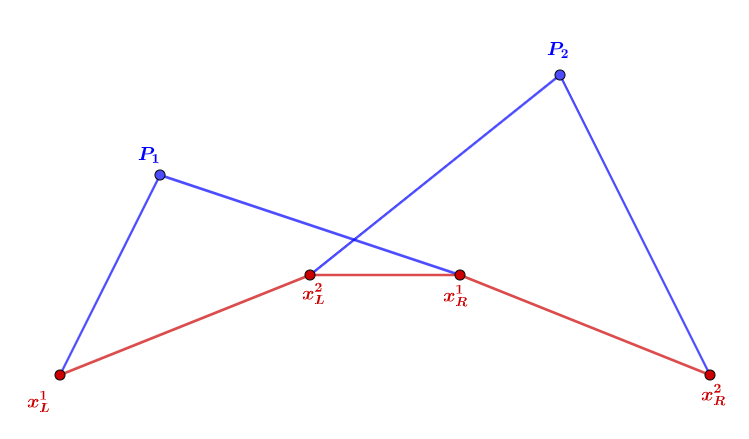
\includegraphics[width = 0.7\linewidth]{proof1.PNG}
%     \caption{The mothership launches two drones sequentially}
%     \label{fig:proof1}
% \end{figure}

% For this result, we can assume that the drone has to visit degenerate graphs into points, otherwise, we can reduce the available capacity so that is possible to traverse the required percentage of these graphs. Without loss of generality, it is also supposed that we only have two target points.  


% \begin{theorem}
% Let $x_L^1$, $x_L^2$ (resp. $x_R^1$, $x_R^2$) be the launch (resp. rendezvous) points associated to the visit of the target points $P_1$ and $P_2$. If there exists $x_L$ and $x_R$ verifying 
% $$
%  \left\{
%  \begin{array}{ccl}
%   \dfrac{\|x_L-x_R\|}{v_C} & \leq    & \dfrac{\|x_L - P_1\| + \|P_1 - x_R\|}{v_D} \\
%   \dfrac{\|x_L-x_R\|}{v_C} & \leq    & \dfrac{\|x_L - P_2\| + \|P_2 - x_R\|}{v_D} \\
%   \dfrac{\|x_L-x_R\|}{v_C} & \leq   & capacity \\
%   \|x_L-x_R\| & \leq & \|x_L^1 - x_L^2\| + \|x_L^2- x_R^1\| + \|x_R^1-x_R^2\|
%  \end{array}
%  \right.
% $$

% then both models provide the same objective value in the optimal solution.
% \end{theorem}

% \begin{proof}
% Note that, since the binary variables are fixed in this case, the only difference than models can have are the location of the launch and rendezvous points. Hence, the only involved constraints are those related to these points. The first two are the \eqref{DCW} inequalities. The third one is the \eqref{CAP} constraint and the last one ensures that the distance made by the mothership for the synchonisation case is lower than the distance given in the hypothesis of the statement.

% \end{proof}

% Note that this result states necessary and sufficient conditions to obtain the same solution for the two models.


%(Meto restricción de capacidad? para hacer experimentos puede complicarse)

% $$
% e=(i, j) \ni x_R^o \rightarrow V_i \vee V_j \rightarrow \ldots \rightarrow V_k \rightarrow \ldots \rightarrow V_{i'} \rightarrow x_L^{t+1} \in (i',j')=e'
% $$

% The design of these paths obeys to define binary variables that decide which vertices are selected in each stage $t$: 